\documentclass[kulak]{tplt} 
% options: kulak (default) or kul

\title{Algebraic Methods in Combinatorics}
\author{Solution to assignment 0}
\date{Summer semester 2022 -- 2023}
\address{
	\textbf{Max Planck Institute for the Mathematics in the Sciences} \\
	\textbf{Universit\"at Leipzig}}


\usepackage{graphicx}
\usepackage{amssymb}
\usepackage{amsthm}
\usepackage{bbold}
\usepackage{listings}
\usepackage{lineno}
%\usepackage[margin=3cm]{geometry}
\usepackage[all,cmtip, color,matrix,arrow]{xy}
%\usepackage{amsaddr}
\usepackage{tikz-cd}
\usepackage{amsmath}%To use \text 
\usepackage[utf8]{inputenc}
\usepackage{hyperref}
\usepackage[capitalize]{cleveref}
\crefname{thm}{Theorem}{Theorems}
%\usepackage{bbold}
\usepackage[export]{adjustbox}
\usepackage{todonotes}
\usepackage{bm}
\usepackage{wrapfig}
\usepackage{float}
\usepackage{mathtools}
\usepackage{aliascnt}
\newaliascnt{eqfloat}{equation}
\newfloat{eqfloat}{h}{eqflts}
\floatname{eqfloat}{Equation}
\usepackage{dirtytalk}
\usepackage[mathscr]{euscript}


%\def\shuffle{\sqcup\mathchoice{\mkern-7mu}{\mkern-7mu}{\mkern-3.2mu}{\mkern-3.8mu}\sqcup\,}
\newcommand{\qshuffle}{\overline{\shuffle}}


\theoremstyle{definition}
\newtheorem{thm}{Theorem}[section]
\newtheorem{prop}[thm]{Proposition}
\newtheorem{lm}[thm]{Lemma}
\newtheorem{cor}[thm]{Corollary}
\newtheorem{obs}[thm]{Observation}
\newtheorem{defin}[thm]{Definition}
\newtheorem{smpl}[thm]{Example}
\newtheorem{quest}[thm]{Question}
\newtheorem{exe}[thm]{Exercise}
\newtheorem{const}[thm]{Construction}
\newtheorem{prob}[thm]{Problem}
\newtheorem{conj}[thm]{Conjecture}
\newtheorem{rem}[thm]{Remark}
\crefname{lm}{Lemma}{Lemmas}
\crefname{thm}{Theorem}{Theorems}
\crefname{prop}{Proposition}{Propositions}
\crefname{defin}{Definition}{Definitions}
\crefname{rem}{Remark}{Remarks}

\newcommand{\R}{\mathbb{R}}
\newcommand{\Z}{\mathbb{Z}}
\newcommand{\F}{\mathbb{F}}
\newcommand{\Q}{\mathbb{Q}}
\newcommand{\PP}{\mathbb{P}}

\newcommand{\one}{\mathbb{1}}

\newcommand{\CC}{\mathcal C}
\newcommand{\JJ}{\mathcal J}
\newcommand{\II}{\mathcal I}
\newcommand{\BB}{\mathcal B}
\newcommand{\FF}{\mathcal F}

%vectors
\newcommand{\vv}{\mathsf{v}}
\newcommand{\vw}{\mathsf{w}}
\newcommand{\vj}{\mathsf{j}}
\newcommand{\vx}{\mathsf{x}}
\newcommand{\vy}{\mathsf{y}}
\newcommand{\va}{\mathsf{a}}

\newcommand{\spn}{\mathrm{span}}
\newcommand{\rk}{\mathrm{rk}}
\newcommand{\tr}{\mathrm{tr}}
\newcommand{\conv}{\mathrm{conv}}
\newcommand{\maxcut}{\mathrm{maxcut}}
\newcommand{\we}{\mathrm{we}}


\begin{document}

\maketitle
\begin{enumerate}
\item 

The maximal number of clubs in Oddtown and in Eventown is, respectively, 
$$\sum_{\substack{k=0\\ k \text{ odd }}}^{10} \binom{10}{k} \text{ and }\sum_{\substack{k=0\\ k \text{ even }}}^{10} \binom{10}{k}\, . $$

These sums can be evaluated more explicitly in several ways.
We present here a method using the \textbf{binomial identity} $(x+y)^n = \sum_{k=0}^n \binom{n}{k} x^ky^{n-k}$.
Set $n = 10, x = 1$ and $y = 1$ to get
$$ 1024 = 2^{10} = \sum_{k = 0}^{10}\binom{10}{k}\, . $$

Set $n = 10, x = 1$ and $y = -1$ to get
$$ 0 = 0^{10} = \sum_{k = 0}^{10}\binom{10}{k}(-1)^k \, . $$

Taking the sum of both equations gives us
$$ 1024 = \sum_{\substack{k=0\\ k \text{ even }}}^{10} \binom{10}{k}2\, ,$$
and taking the difference of both sums gives us
$$ 1024 = \sum_{\substack{k=0\\ k \text{ odd }}}^{10} \binom{10}{k}2\, ,$$
so we conclude that the maximal number of clubs in each town is $512 = 1024 / 2$.


\item 
The picture in \cref{fig:plane_chromat} shows a graph that can be embedded in the plane, in such a way that the image of any two neighbouring vertices is at distance one of each other.

This graph cannot be coloured with two colours in a proper way, so the plane cannot be coloured with two colours in a proper way.

A proper colouring of the plane using seven colours is sketched in \cref{fig:plane_chromat}.

%\begin{figure}[h]
%\centering
%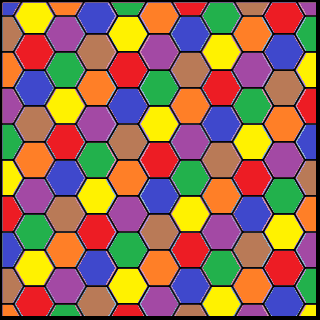
\includegraphics[scale=0.3]{../imgs/plane_chromat7.png}
%\caption{\label{fig:plane_chromat7}}
%\end{figure}

\begin{figure}[h]
\centering
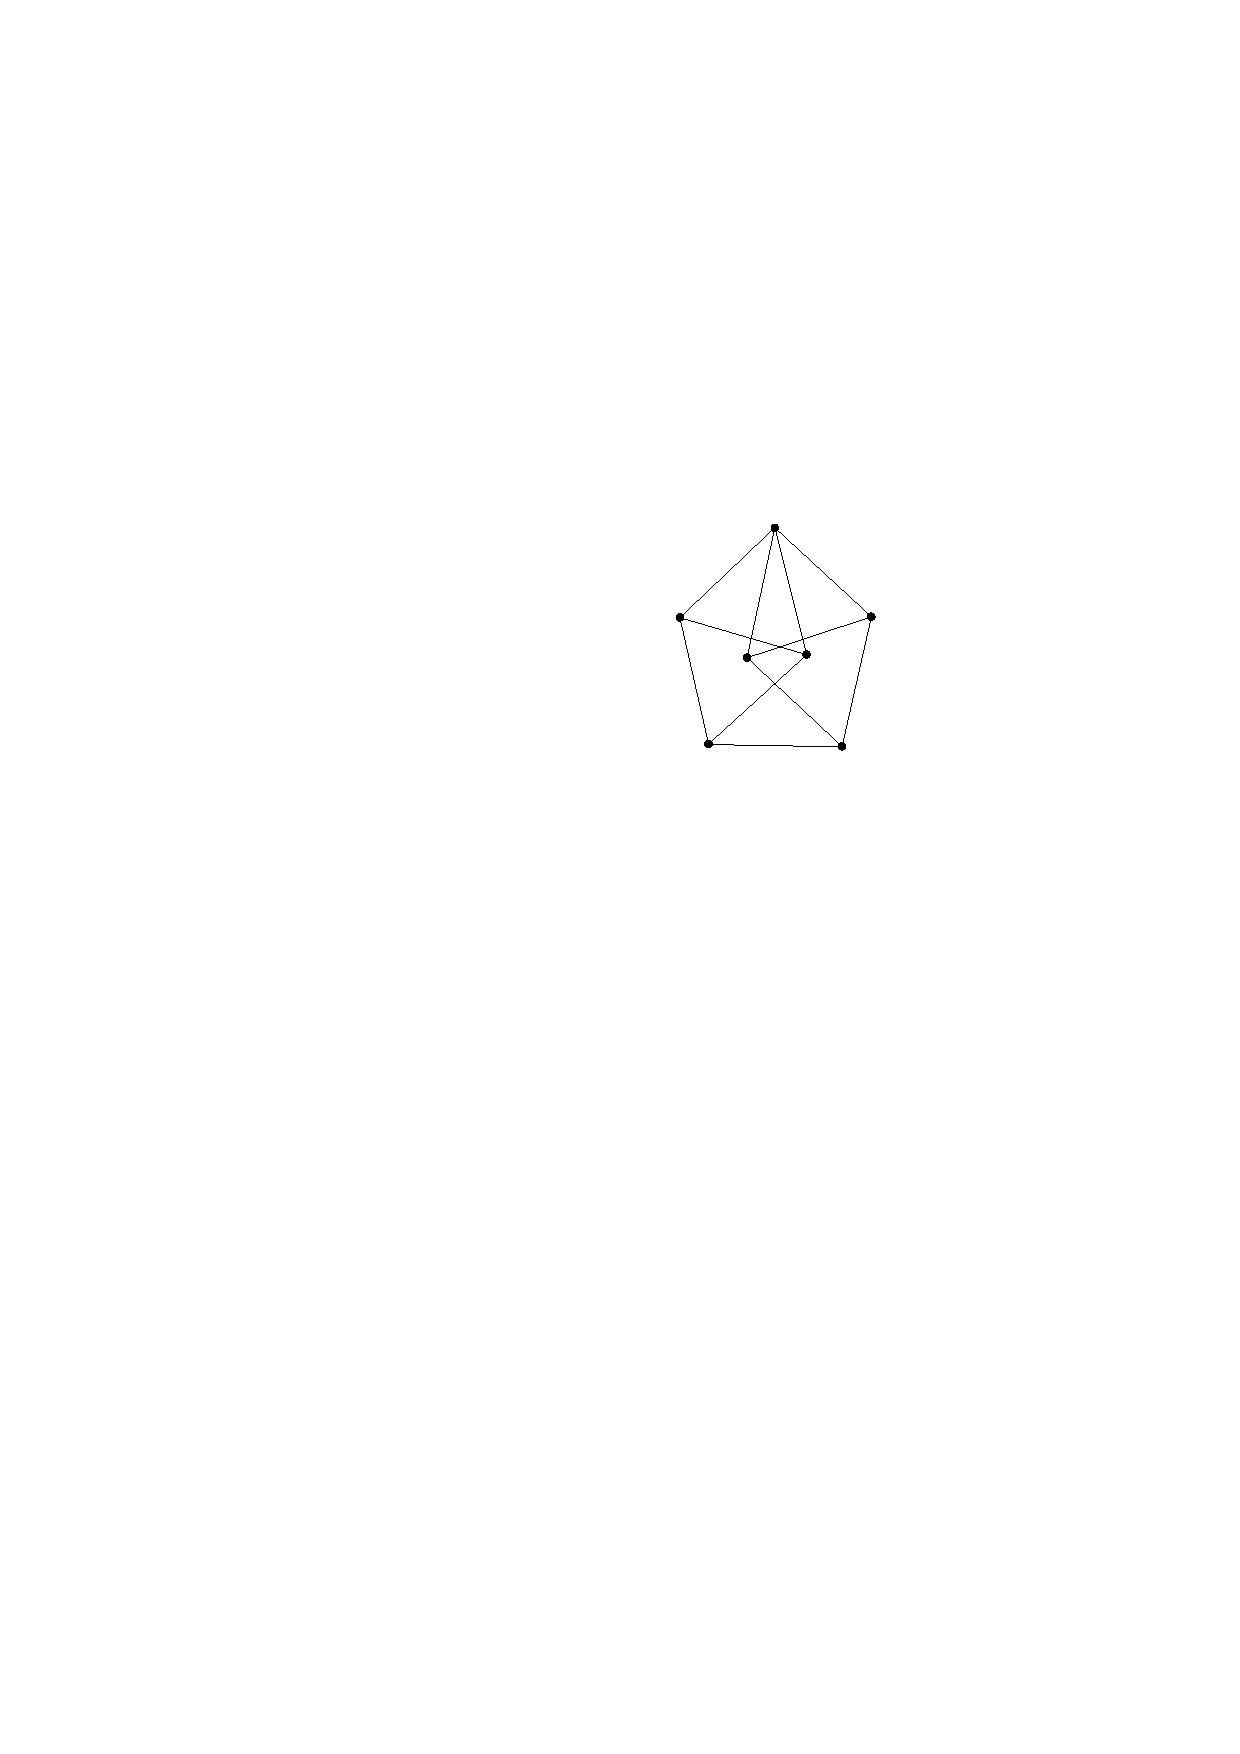
\includegraphics[scale=0.7]{../imgs/plane_chromat}
\hspace{2cm}
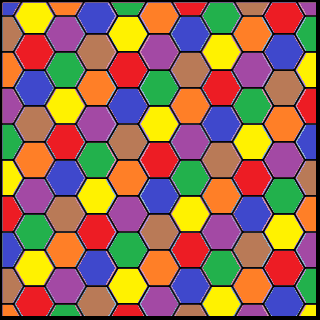
\includegraphics[scale=0.3]{../imgs/plane_chromat7.png}
\caption{\textbf{Left} A graph with chromatic number three, that can be isometrically embedded in the plane. \textbf{Right} A proper colouring of the plane using seven colours.\label{fig:plane_chromat}}
\end{figure}


\item 
Fix a vertex $v$ of the graph, and consider $\{v_1, \dots, v_r\}$ its neighbours.
Note that any vertex $w$ that is a neighbour of both $v_i, v_j$, for $i, j$, distinct, forms a cycle of length four
$$ w - v_i - v - v_j $$
which is impossible because the girth of the graph is five.
Thus this cycle is not proper, that is there are some repeated vertices, which can only be $w = v$.
We conclude that all the neighbours of $v_i, v_j$, other than $v$, are distinct.
Counting all such vertices we get
$$ \underbrace{1}_{\text{ vertex $v$ }} + \underbrace{r}_{v_1, \ldots , v_r} + \underbrace{r(r-1)}_{\text{ each neighbour of $v_i$ distinct from $v$}} = 1 + r^2 \, .$$
\end{enumerate}
\end{document}
